%-------------------------------------------------
\begin{frame}{Beyond Black-box Optimization}
\medskip
Recall general blackbox optimization:\\
        \bigskip
        \begin{center}
        \scalebox{0.7}{\hspace*{1.0cm}
        \newcommand{\myblackbox}{\fcolorbox{black}{black}{
    \minipage[t]{\dimexpr0.111\linewidth-2\fboxsep-2\fboxrule\relax}
        ~~~\\
        ~~~\\
        ~~~\\
    \endminipage}}
    
    
    	\begin{tikzpicture}
\tikzstyle{every node}=[draw,fill=white,minimum width=0cm,thin]
\tikzstyle{every path}=[-latex,ultra thick]
\node (A) [draw=white]{{\Huge{$\conf$}}};
\node (B) [right=14mm of A,draw=white] {\myblackbox{}};
\node (C) [right=14mm of B,draw=white] {{\Huge{$f(\conf)$}}};
%\node (D) [below=7mm of B, align=center, fill=black!10] {\large{Bayesian}\\\large{optimization}};

\draw ($(A.east)+(0.2,0.0)$) -- ($(B.west)+(-0.2,0.0)$);
\draw ($(B.east)+(0.2,0.0)$) -- ($(C.west)+(-0.2,0.0)$);
%\draw ($(C.south)+(0.0,-0.2)$) -| ++(0.0,0.0) |- ($(D.east)+(0.2,0.0)$);
%\draw ($(D.west)+(-0.2,0.0)$) |- ++(0.0,0.0) -| ($(A.south)+(0.0,-0.2)$);
\end{tikzpicture}
}\\
        \bigskip
         Only mode of interaction with $f$: querying $f$'s value at a given $\conf$
        
\pause
        \bigskip
        \bigskip
        \huge{\textcolor{red}{Too slow for tuning expensive models}}
        
        \end{center}
\vspace*{-6cm}
\begin{center}
\scalebox{15}{\color{Red}{$\bm{\times}$}}
\end{center}    
    
\end{frame}
%-------------------------------------------------

%-------------------------------------------------
%  \begin{frame}{Outline}
%    \bigskip
%    \vfill
%    \tableofcontents
%  \end{frame}
%-------------------------------------------------

\begin{frame}[c]{Methods for Going Beyond Blackbox Bayesian Optimization}

\begin{columns}

    \column{0.5\textwidth}
    \begin{itemize}
        \item One possible cheap approximation of an expensive function: use a data subset
        \begin{itemize}
            \item Many cheap evaluations on small subsets
            \item Few expensive evaluations on the full data
        \end{itemize}
    \end{itemize}
    
    \column{0.5\textwidth}
    \begin{figure}
        \centering
        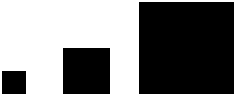
\includegraphics[width=0.3\textwidth]{w07_hpo_grey_box/images/intro/black_blocks.png}
    \end{figure}

\end{columns}

\begin{itemize}
    \item E.g.: Support Vector Machines (SVM) on MNIST dataset (hyperparameters: C, $\gamma$)
\end{itemize}

% Screen shots were clipped to 114, 500, 1860, 940
\only<1>{
    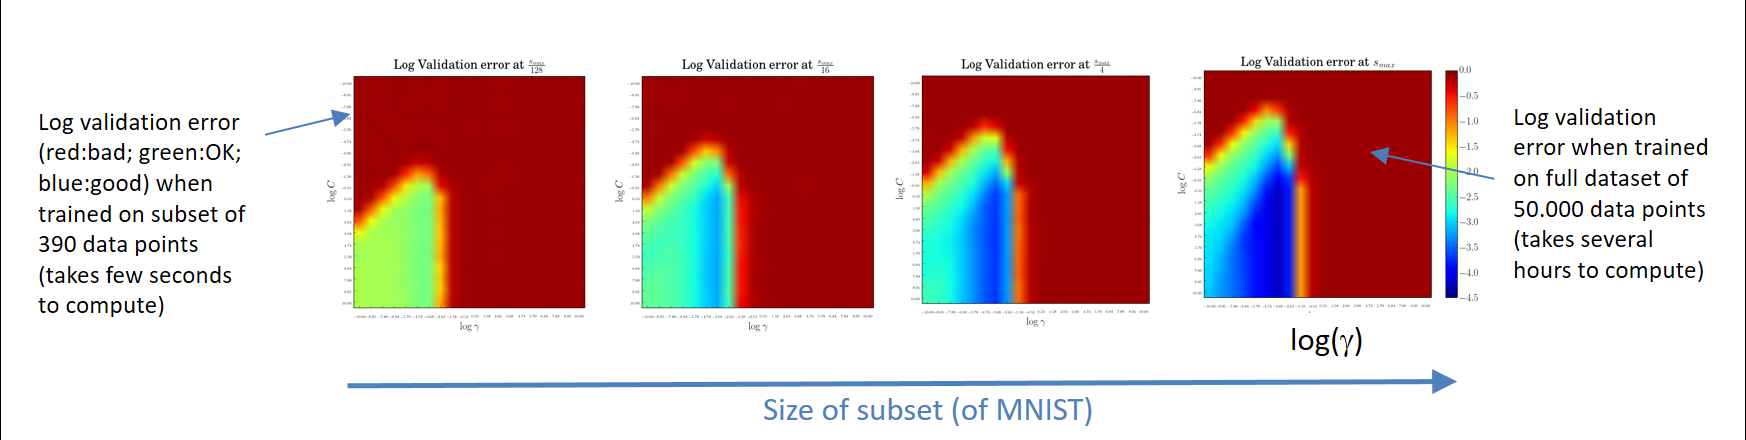
\includegraphics[width=\textwidth,trim=5px 10px 5px 10px, clip]{w07_hpo_grey_box/images/intro/animation_1.png}
}

\only<2->{
    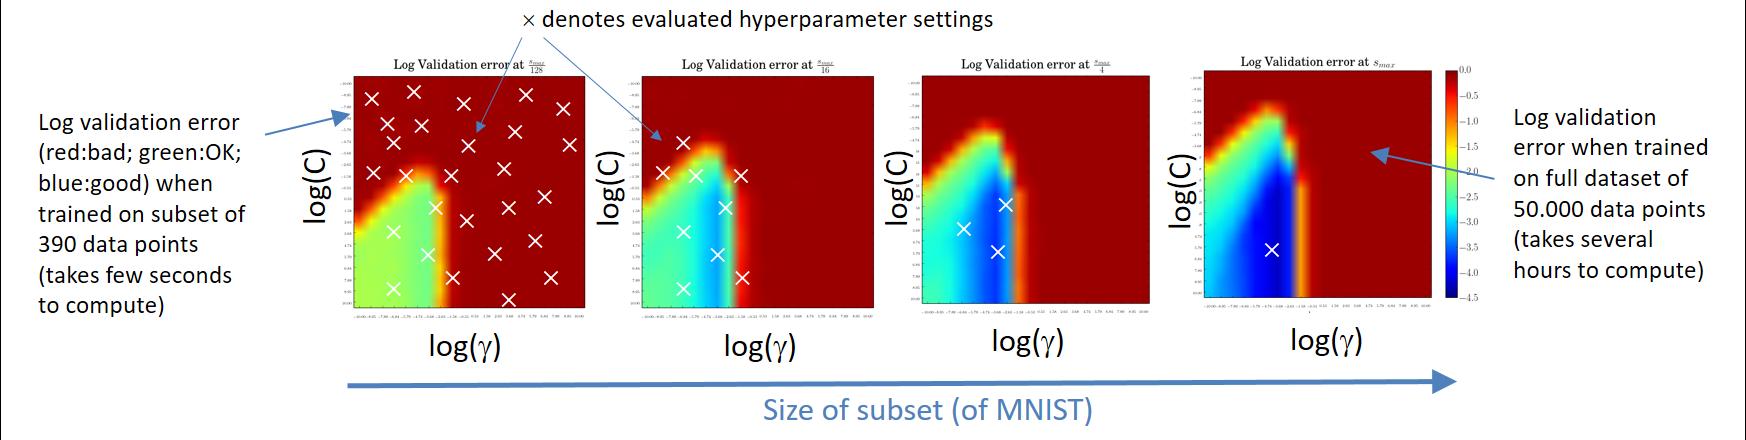
\includegraphics[width=\textwidth,trim=5px 10px 5px 10px, clip]{w07_hpo_grey_box/images/intro/animation_2.png}
}

\vskip -15pt

\only<3->{
    $\rightarrow$ up to 1000x speedups over blackbox optimization on full data \lit{\href{http://proceedings.mlr.press/v54/klein17a/klein17a.pdf}{Klein et al, AISTATS 2017}}
}

\end{frame}

%-----------------------------------------------------------------------

\begin{frame}[c]{Learning Goals of this Lecture}
\framesubtitle{After this lecture, students can ...}

\begin{itemize}
    \item Describe many different ways of using \alert{meta-learning} to speed up HPO
    \item Discuss several ways of predicting \alert{learning curves}
    \item Explain how to \alert{exploit multiple fidelities in Bayesian optimization} 
    \item Explain the \alert{Successive Halving} and \alert{Hyperband} algorithms 
    \item Explain how to combine Bayesian optimization and Hyperband in \alert{BOHB}
    \item Discuss \alert{success stories} of speeding up Bayesian optimization
\end{itemize}
\end{frame}

%-----------------------------------------------------------------------











%-------------------------------------------------
\iffalse


%-------------------------------------------------
\begin{frame}{Recall: Black-box optimization}

\begin{figure}
    \centering
    


\tikzset{every picture/.style={line width=0.75pt}} %set default line width to 0.75pt        

\begin{tikzpicture}[x=0.70pt,y=0.70pt,yscale=-1,xscale=1]
%uncomment if require: \path (0,300); %set diagram left start at 0, and has height of 300

%Straight Lines [id:da5075678478287002] 
\draw    (74.5,104) -- (218.5,104) ;
\draw [shift={(220.5,104)}, rotate = 180] [color={rgb, 255:red, 0; green, 0; blue, 0 }  ][line width=0.75]    (10.93,-3.29) .. controls (6.95,-1.4) and (3.31,-0.3) .. (0,0) .. controls (3.31,0.3) and (6.95,1.4) .. (10.93,3.29)   ;
%Shape: Square [id:dp6368535923226633] 
\draw  [fill={rgb, 255:red, 0; green, 25; blue, 255 }  ,fill opacity=1 ] (14,79) -- (64,79) -- (64,129) -- (14,129) -- cycle ;
%Shape: Square [id:dp8011400143211207] 
\draw  [fill={rgb, 255:red, 0; green, 25; blue, 255 }  ,fill opacity=1 ] (561,79) -- (611,79) -- (611,129) -- (561,129) -- cycle ;
%Straight Lines [id:da6772752516220095] 
\draw    (401.5,101) -- (540.5,101.99) ;
\draw [shift={(542.5,102)}, rotate = 180.41] [color={rgb, 255:red, 0; green, 0; blue, 0 }  ][line width=0.75]    (10.93,-3.29) .. controls (6.95,-1.4) and (3.31,-0.3) .. (0,0) .. controls (3.31,0.3) and (6.95,1.4) .. (10.93,3.29)   ;
%Straight Lines [id:da7102938160527976] 
\draw    (39.5,242) -- (39.01,143) ;
\draw [shift={(39,141)}, rotate = 449.72] [color={rgb, 255:red, 0; green, 0; blue, 0 }  ][line width=0.75]    (10.93,-3.29) .. controls (6.95,-1.4) and (3.31,-0.3) .. (0,0) .. controls (3.31,0.3) and (6.95,1.4) .. (10.93,3.29)   ;
%Straight Lines [id:da5275375794470956] 
\draw    (39.5,242) -- (123.5,242) ;
%Straight Lines [id:da11206880859629287] 
\draw    (123.5,242) -- (586.5,242) ;
%Straight Lines [id:da8957848321230528] 
\draw    (586.5,135) -- (586.5,242) ;
%Image [id:dp5678753924043267] 
\draw (313.5,101.5) node  {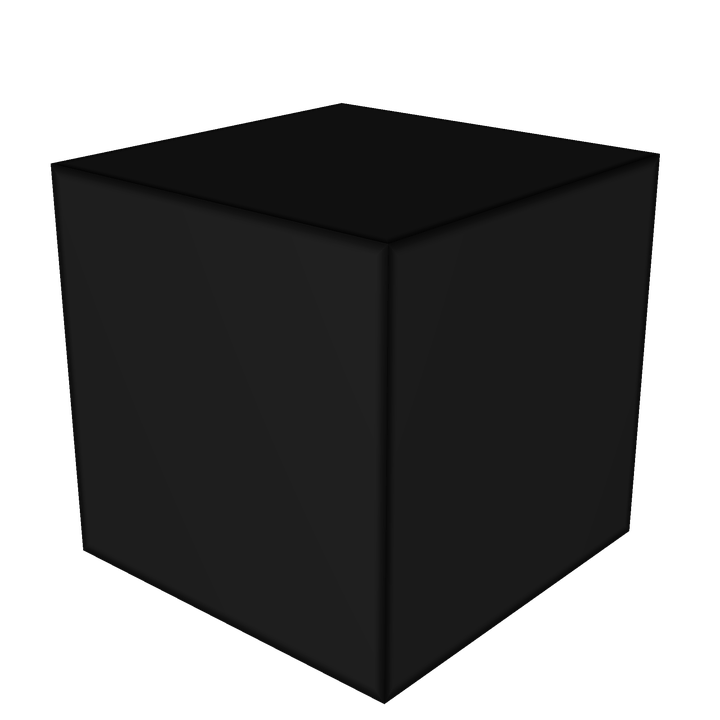
\includegraphics[width=106.5pt,height=104.25pt]{w07_hpo_grey_box/images/intro/black_box.png}};

% Text Node
\draw (284,106.5) node   [align=left] { \textcolor[rgb]{1,1,1}{{\Huge ?}}};
% Text Node
\draw (39,104) node   [align=left] {\textcolor[rgb]{1,1,1}{X}};
% Text Node
\draw (586,102) node   [align=left] {\textcolor[rgb]{1,1,1}{f(X)}};
% Text Node
\draw (317,28) node   [align=left] {Objective function};
% Text Node
\draw (309,254) node   [align=left] {Only interaction: Query of function at $\displaystyle \conf$ to obtain $\displaystyle \cost(\conf)$};


\end{tikzpicture}

\end{figure}
\pause
\begin{itemize}
    \item Can we do better?
\end{itemize}
%\source{\lit{\href{https://slideslive.com/38917532/greybox-bayesian-optimization-for-automl}{Peter Frazier: Grey-box Bayesian Optimization for AutoML}}}
    
    \textcolor{red}{FH: can you please create this figure yourself, using the same picture for black box and looking inside the black box, except that for ``looking inside'' the lid is open. For one (not necessarily optimal) way to do this in tikz, see: http://www.texample.net/tikz/examples/annotated-3d-box/}
    
\end{frame}
%-------------------------------------------------




%\section{Introduction to grey-box approaches}
%-------------------------------------------------
%-------------------------------------------------
\begin{frame}{Recall: Black-box optimization}
\begin{figure}
    \centering
    


\tikzset{every picture/.style={line width=0.75pt}} %set default line width to 0.75pt        

\begin{tikzpicture}[x=0.70pt,y=0.70pt,yscale=-1,xscale=1]
%uncomment if require: \path (0,300); %set diagram left start at 0, and has height of 300

%Straight Lines [id:da5075678478287002] 
\draw    (74.5,104) -- (218.5,104) ;
\draw [shift={(220.5,104)}, rotate = 180] [color={rgb, 255:red, 0; green, 0; blue, 0 }  ][line width=0.75]    (10.93,-3.29) .. controls (6.95,-1.4) and (3.31,-0.3) .. (0,0) .. controls (3.31,0.3) and (6.95,1.4) .. (10.93,3.29)   ;
%Shape: Square [id:dp6368535923226633] 
\draw  [fill={rgb, 255:red, 0; green, 25; blue, 255 }  ,fill opacity=1 ] (14,79) -- (64,79) -- (64,129) -- (14,129) -- cycle ;
%Shape: Square [id:dp8011400143211207] 
\draw  [fill={rgb, 255:red, 0; green, 25; blue, 255 }  ,fill opacity=1 ] (561,79) -- (611,79) -- (611,129) -- (561,129) -- cycle ;
%Straight Lines [id:da6772752516220095] 
\draw    (401.5,101) -- (540.5,101.99) ;
\draw [shift={(542.5,102)}, rotate = 180.41] [color={rgb, 255:red, 0; green, 0; blue, 0 }  ][line width=0.75]    (10.93,-3.29) .. controls (6.95,-1.4) and (3.31,-0.3) .. (0,0) .. controls (3.31,0.3) and (6.95,1.4) .. (10.93,3.29)   ;
%Straight Lines [id:da7102938160527976] 
\draw    (39.5,242) -- (39.01,143) ;
\draw [shift={(39,141)}, rotate = 449.72] [color={rgb, 255:red, 0; green, 0; blue, 0 }  ][line width=0.75]    (10.93,-3.29) .. controls (6.95,-1.4) and (3.31,-0.3) .. (0,0) .. controls (3.31,0.3) and (6.95,1.4) .. (10.93,3.29)   ;
%Straight Lines [id:da5275375794470956] 
\draw    (39.5,242) -- (123.5,242) ;
%Straight Lines [id:da11206880859629287] 
\draw    (123.5,242) -- (586.5,242) ;
%Straight Lines [id:da8957848321230528] 
\draw    (586.5,135) -- (586.5,242) ;
%Image [id:dp5678753924043267] 
\draw (313.5,101.5) node  {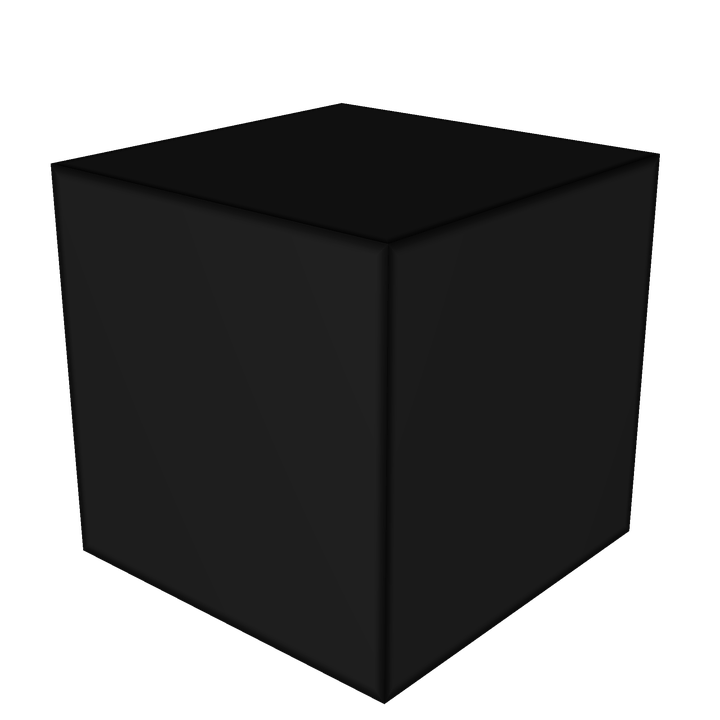
\includegraphics[width=106.5pt,height=104.25pt]{w07_hpo_grey_box/images/intro/black_box.png}};

% Text Node
\draw (284,106.5) node   [align=left] { \textcolor[rgb]{1,1,1}{{\Huge ?}}};
% Text Node
\draw (39,104) node   [align=left] {\textcolor[rgb]{1,1,1}{X}};
% Text Node
\draw (586,102) node   [align=left] {\textcolor[rgb]{1,1,1}{f(X)}};
% Text Node
\draw (317,28) node   [align=left] {Objective function};
% Text Node
\draw (309,254) node   [align=left] {Only interaction: Query of function at $\displaystyle \conf$ to obtain $\displaystyle \cost(\conf)$};


\end{tikzpicture}

\end{figure}
\pause
\begin{itemize}
    \item Can we do better?
\end{itemize}
%\source{\lit{\href{https://slideslive.com/38917532/greybox-bayesian-optimization-for-automl}{Peter Frazier: Grey-box Bayesian Optimization for AutoML}}}
    
    \textcolor{red}{FH: can you please create this figure yourself, using the same picture for black box and looking inside the black box, except that for ``looking inside'' the lid is open. For one (not necessarily optimal) way to do this in tikz, see: http://www.texample.net/tikz/examples/annotated-3d-box/}
    
\end{frame}
%-------------------------------------------------
%-------------------------------------------------
\begin{frame}{Looking inside the box}
\begin{figure}
    \centering
    


\tikzset{every picture/.style={line width=0.75pt}} %set default line width to 0.75pt        

\begin{tikzpicture}[x=0.70pt,y=0.70pt,yscale=-1,xscale=1]
%uncomment if require: \path (0,300); %set diagram left start at 0, and has height of 300

%Straight Lines [id:da5075678478287002] 
\draw    (74.5,104) -- (218.5,104) ;
\draw [shift={(220.5,104)}, rotate = 180] [color={rgb, 255:red, 0; green, 0; blue, 0 }  ][line width=0.75]    (10.93,-3.29) .. controls (6.95,-1.4) and (3.31,-0.3) .. (0,0) .. controls (3.31,0.3) and (6.95,1.4) .. (10.93,3.29)   ;
%Shape: Square [id:dp6368535923226633] 
\draw  [fill={rgb, 255:red, 0; green, 25; blue, 255 }  ,fill opacity=1 ] (14,79) -- (64,79) -- (64,129) -- (14,129) -- cycle ;
%Shape: Square [id:dp8011400143211207] 
\draw  [fill={rgb, 255:red, 0; green, 25; blue, 255 }  ,fill opacity=1 ] (561,79) -- (611,79) -- (611,129) -- (561,129) -- cycle ;
%Straight Lines [id:da6772752516220095] 
\draw    (401.5,101) -- (540.5,101.99) ;
\draw [shift={(542.5,102)}, rotate = 180.41] [color={rgb, 255:red, 0; green, 0; blue, 0 }  ][line width=0.75]    (10.93,-3.29) .. controls (6.95,-1.4) and (3.31,-0.3) .. (0,0) .. controls (3.31,0.3) and (6.95,1.4) .. (10.93,3.29)   ;
%Straight Lines [id:da7102938160527976] 
\draw    (39.5,242) -- (39.01,143) ;
\draw [shift={(39,141)}, rotate = 449.72] [color={rgb, 255:red, 0; green, 0; blue, 0 }  ][line width=0.75]    (10.93,-3.29) .. controls (6.95,-1.4) and (3.31,-0.3) .. (0,0) .. controls (3.31,0.3) and (6.95,1.4) .. (10.93,3.29)   ;
%Straight Lines [id:da5275375794470956] 
\draw    (39.5,242) -- (123.5,242) ;
%Straight Lines [id:da11206880859629287] 
\draw    (123.5,242) -- (586.5,242) ;
%Straight Lines [id:da8957848321230528] 
\draw    (586.5,135) -- (586.5,242) ;
%Image [id:dp9410017568713034] 
\draw (307.5,95) node  {
\includegraphics[width=94.5pt,height=76.5pt]{w07_hpo_grey_box/images/intro/opened_box.png}};
%Straight Lines [id:da7498039648909043] 
\draw    (264,72) -- (222.18,45.08) ;
\draw [shift={(220.5,44)}, rotate = 392.77] [color={rgb, 255:red, 0; green, 0; blue, 0 }  ][line width=0.75]    (10.93,-3.29) .. controls (6.95,-1.4) and (3.31,-0.3) .. (0,0) .. controls (3.31,0.3) and (6.95,1.4) .. (10.93,3.29)   ;

% Text Node
\draw (39,104) node   [align=left] {\textcolor[rgb]{1,1,1}{X}};
% Text Node
\draw (586,102) node   [align=left] {\textcolor[rgb]{1,1,1}{f(X)}};
% Text Node
\draw (317,28) node   [align=left] {Objective function};
% Text Node
\draw (309,254) node   [align=left] {Only interaction: Query of function at $\displaystyle \conf$ to obtain $\displaystyle \cost(\conf)$};
% Text Node
\draw (158,38) node   [align=left] {other information};


\end{tikzpicture}

\end{figure}

    \textcolor{red}{FH: can you please create this figure yourself, using the same picture for black box and looking inside the black box, except that for ``looking inside'' the lid is open. For one (not necessarily optimal) way to do this in tikz, see: http://www.texample.net/tikz/examples/annotated-3d-box/}

%\hspace{6.5cm}\lit{\href{https://slideslive.com/38917532/greybox-bayesian-optimization-for-automl}{Peter Frazier: Grey-box Bayesian Optimization for AutoML}}
\end{frame}
%-------------------------------------------------


\begin{frame}{Looking inside the box}
Utilize additional knowledge available about the objective function to improve optimization performance:
\begin{itemize}
    \item Learning curves:
    \begin{itemize}
        \item Early stopping
        \item Freezing \& Thawing
    \end{itemize}
    \item Cheap-to-evaluate proxies
    \begin{itemize}
        \item Trained neural network on small part of $\dataset$ 
    \end{itemize}
    \item Multi-task learning
    \begin{itemize}
        \item Solve multiple learning tasks simultaneously.
        \item Exploit commonalities and differences across tasks.
    \end{itemize}
    \item Warm starts
    \begin{itemize}
        \item Reuse trained hyperparameter configurations from similar models or datasets.
    \end{itemize}
\end{itemize}
\end{frame}
%-------------------------------------------------
%-------------------------------------------------
%\iffalse
\begin{frame}{Learning Curves}

\centering
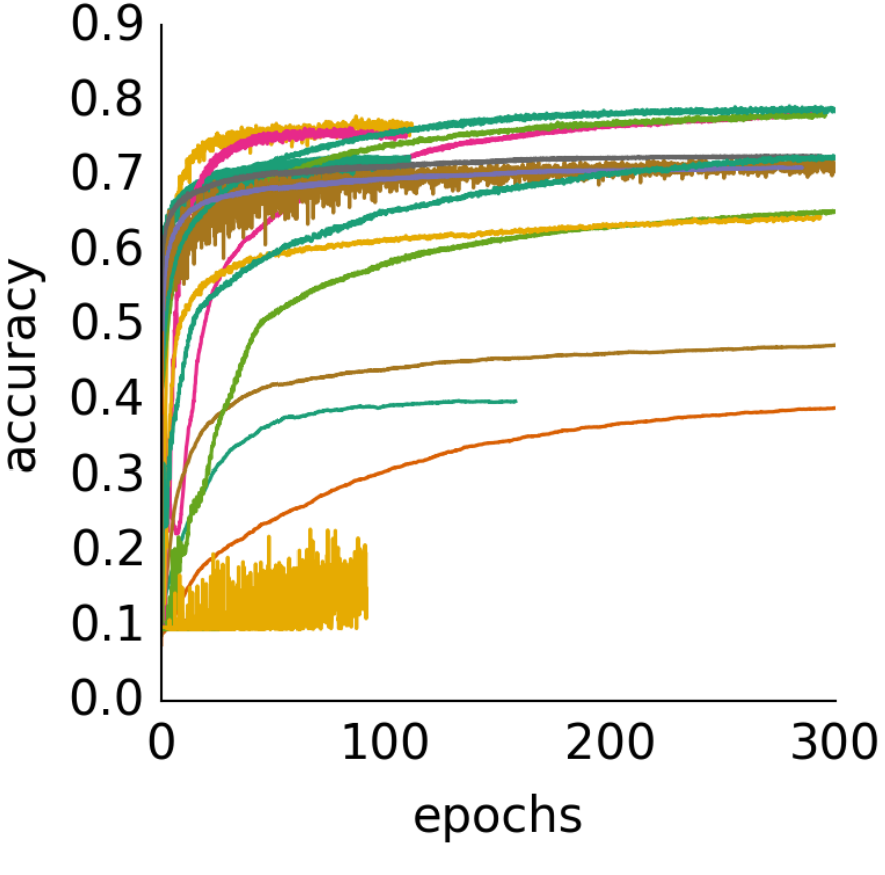
\includegraphics[width=0.4\textwidth]{w07_hpo_grey_box/images/intro/learning_curves.png}

Exemplary learning curves of training deep neural networks\\
Many ML algorithms iteratively optimize a (loss) function

\end{frame}
%-------------------------------------------------
%-------------------------------------------------
\begin{frame}{Stopping poor evaluations early}

\centering
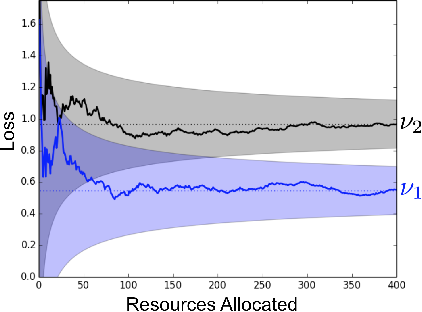
\includegraphics[width=0.5\textwidth]{w07_hpo_grey_box/images/intro/differetiatingConfigurations.png}

Only stop evaluations after they have spent sufficient resources to differentiate between them in terms of quality.

\end{frame}
\fi